\section{Forward-Backward Algorithm}
\subsection{Background}
A Markov chains is a stochastic model in which future events can be predicted due to the fact that the probability of an event depends only on the state attained in the previous event. Schematically, a hidden Markov model (HMM) can be seen in Fig.\ref{markove_diagram} where $H_1, H_2, ... , H_T$ follow a (first-order stationary) Markov process, the state space is ${s_1, s_2, ... , s_N}$ and the transition probabilities $p_{i,j}$ form the $N \, \textrm{x} \, N$ transition matrix $M$. Thus the initial probabilities are defined as $p_i = \textrm{Pr}(H_1 = s_i ), i = 1, 2, ... , N$. We observe $V_1 V_2, ... $ and given the value of $H_t$, the variable $V_t$ is the observable, independent of
everything else. The possible values of $V_t$ are defined as ${x_1, x_2, ... x_k}$ where the distribution is given by emission probabilities. $b_{i,k} = \textrm{Pr}(V_t = x_k | H_t = s_i )$ that form the $N \, \textrm{x} \, K$ emission
matrix $B$. This is what is known as a HMM.



\begin{figure}[ht] 				
 % Figure placement: [h]ere, [t]op, [b]ottom, or [p]age
   \centering											% Center in the column
   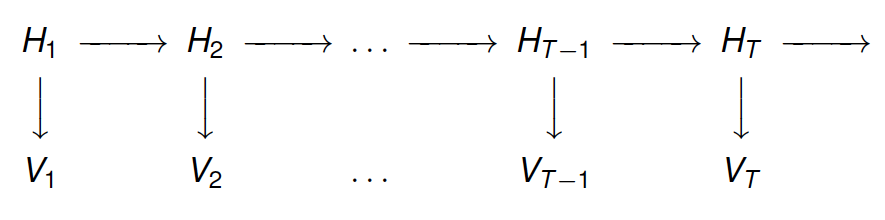
\includegraphics[width=8cm]{Figures/markov_process.png} 			% Command to include the graphics file 
   \caption{Schematic representation of a (first-order stationary) hidden Markov Model.}		% Caption
   \label{markove_diagram}								% Label so the figure can be referred to before or later
\end{figure}

\subsection{Algorithm}
Suppose the parameters of a HMM are known and we have
observed $v_1, v_2, ... ,v_T$, now we can calculate 
\begin{equation}\label{fwcal}
\textrm{Pr}(H_t=s_i|v_1,...,v_T).
\end{equation}
The Forward-Backward Algorithm is an implementation of dynamic programming used to calculate Eq.\ref{fwcal} with computational time $O(N^2T)$.

